

\tikzset{every picture/.style={line width=0.75pt}} %set default line width to 0.75pt        

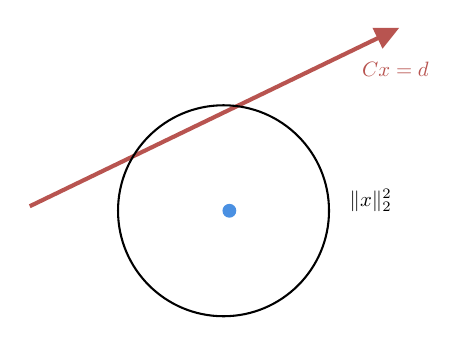
\begin{tikzpicture}[x=0.75pt,y=0.75pt,yscale=-1,xscale=1]
%uncomment if require: \path (0,300); %set diagram left start at 0, and has height of 300

%Straight Lines [id:da6117902046112789] 
\draw [color={rgb, 255:red, 184; green, 84; blue, 80 }  ,draw opacity=1 ][fill={rgb, 255:red, 184; green, 84; blue, 80 }  ,fill opacity=1 ][line width=1.5]    (199,160.65) -- (373.4,76.41) ;
\draw [shift={(377,74.67)}, rotate = 154.22] [fill={rgb, 255:red, 184; green, 84; blue, 80 }  ,fill opacity=1 ][line width=0.08]  [draw opacity=0] (11.61,-5.58) -- (0,0) -- (11.61,5.58) -- cycle    ;
%Shape: Circle [id:dp3140562285855766] 
\draw   (241.53,162.82) .. controls (241.53,134.75) and (264.28,112) .. (292.35,112) .. controls (320.42,112) and (343.18,134.75) .. (343.18,162.82) .. controls (343.18,190.89) and (320.42,213.65) .. (292.35,213.65) .. controls (264.28,213.65) and (241.53,190.89) .. (241.53,162.82) -- cycle ;
%Shape: Circle [id:dp5255822841062723] 
\draw  [color={rgb, 255:red, 74; green, 144; blue, 226 }  ,draw opacity=1 ][fill={rgb, 255:red, 74; green, 144; blue, 226 }  ,fill opacity=1 ] (292.35,162.82) .. controls (292.35,161.26) and (293.62,160) .. (295.18,160) .. controls (296.74,160) and (298,161.26) .. (298,162.82) .. controls (298,164.38) and (296.74,165.65) .. (295.18,165.65) .. controls (293.62,165.65) and (292.35,164.38) .. (292.35,162.82) -- cycle ;

% Text Node
\draw (358,90) node [anchor=north west][inner sep=0.75pt]  [color={rgb, 255:red, 184; green, 84; blue, 80 }  ,opacity=1 ,xscale=0.75,yscale=0.75]  {$Cx=d$};
% Text Node
\draw (352,151.4) node [anchor=north west][inner sep=0.75pt]  [xscale=0.75,yscale=0.75]  {$\| x\| _{2}^{2}$};


\end{tikzpicture}